\subsubsection*{Sequence Diagram}
\label{app:diagram}
Source: \textit{Figure 6: Changing the actual value for MVC} in \cite{fowlergui}

\begin{figure}[H]
	\centering
	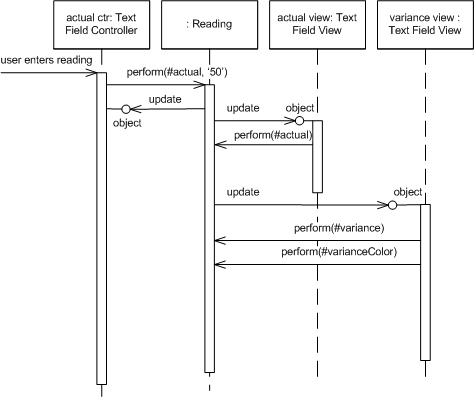
\includegraphics[width=12cm]{images/mvc-seq.png}
	%\caption{The Tool contains Controller and View(s)}
	%\captionsetup{font={footnotesize,bf,it}}
	%\caption*{Source: \cite{reenskaugweb}}
	%\label{fig:tool}
\end{figure}

This sequence diagram demonstrates the change to the value of an input text field. It is used in the thesis to illustrate the different interpretations of the View--Controller relationship. Here, user input is recognized directly by the Controller. In a different intepretation, user input is recognized by the View, which then calls the Controller.

\newpage
\subsubsection*{JSON format of a job description as returned by the log analysis REST service}
\label{app:json}
\inputminted[tabsize=2,linenos]{javascript}{info.json}.